\section{Task: Import ASTERIX Data}
\label{sec:task_import_asterix}

This tash allows importing of ASTERIX data recording files into the opened database. \\

\begin{figure}[H]
  \hspace*{-2.5cm}
    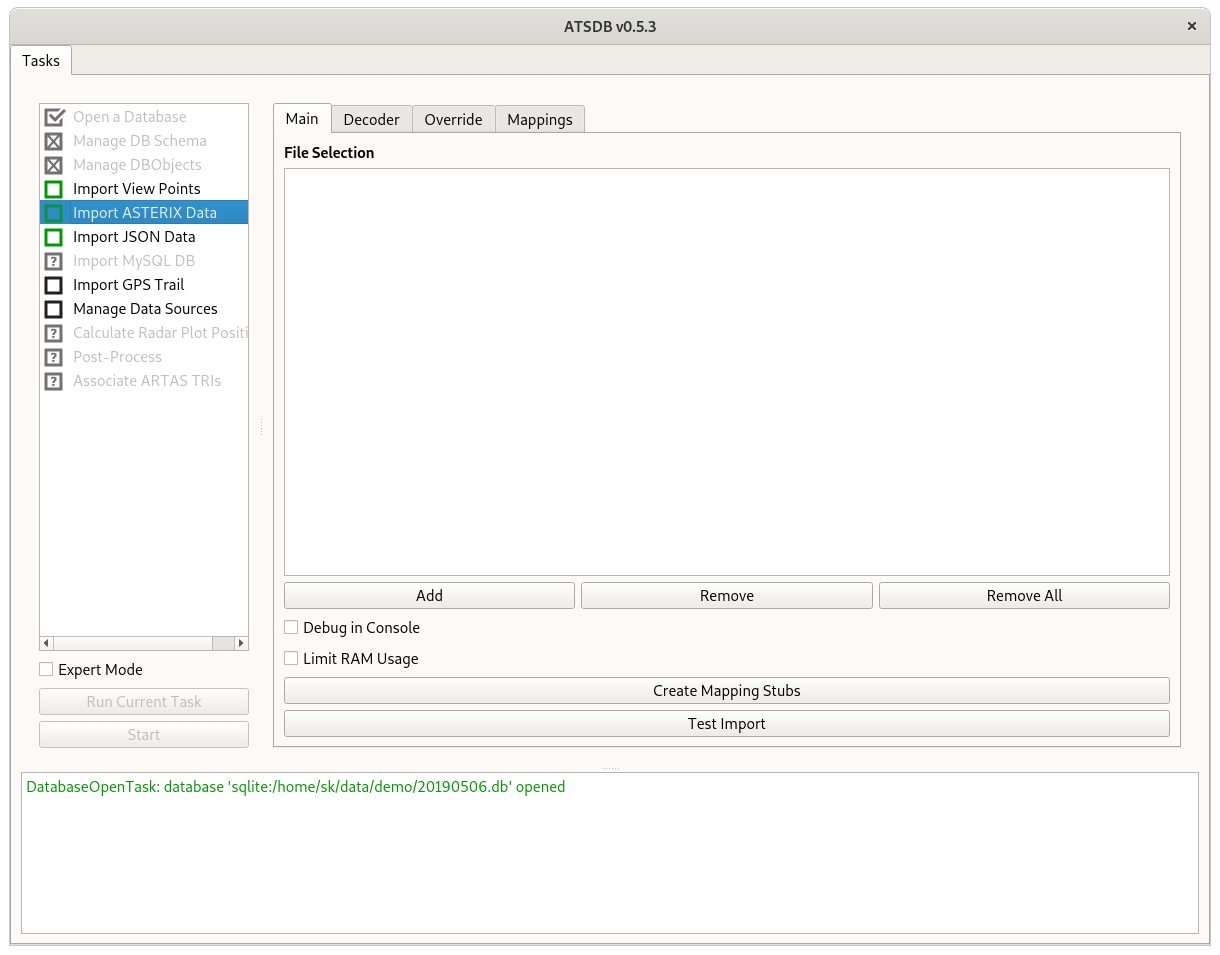
\includegraphics[width=19cm]{../screenshots/asterix_import_data.png}
  \caption{Task: Import ASTERIX data}
\end{figure}

There exist 4 tabs:

\begin{itemize}  
\item Main: File list and support functions/parameters
\item Decoder: jASTERIX decoder settings
\item Override: Tracker data overide settings
\item Mappings: Defintion of created database content based on decoded data
\end{itemize}
\ \\

Please note that the following framings are currently supported:
\begin{itemize}  
\item None: Raw, netto, unframed ASTERIX data blocks
\item IOSS: IOSS Final Format
\item IOSS\_SEQ: IOSS Final Format with sequence numbers
\item RFF: Comsoft RFF format
\end{itemize}
\ \\

Please note that the following ASTERIX categories, editions, reserved expansion fields and special purpose fields are currently supported: \\

\begin{tabular}{ | l | r | r | r |}
\hline
  CAT & Editions & REFs & SPFs  \\ \hline
  001 & 1.1 &  &  \\ \hline
  002 & 1.0 &  &  \\ \hline
  019 & 1.2, 1.3 & & \\ \hline
  020 & 1.5, 1.8 & 1.3 & \\ \hline
  021 & 2.1 & & \\ \hline
  023 & 1.2 & & \\ \hline
  034 & 1.26 & & \\ \hline
  048 & 1.15 & & \\ \hline
  062 & 1.12, 1.16, 1.18 & 1.2 & ARTAS TRIs \\ \hline
  063 & 1.0, 1.1 & & \\ \hline
  065 & 1.2, 1.3 & & \\ \hline
\end{tabular} \\
\  \\

Please note that sensor status messages can be decoded, but are not inserted into the database. Decoding of ASTERIX CAT002 is recommended if CAT001 data is imported, since the timestamps are derived from it (if not available in CAT001).

\subsection{Main Tab}

In the 'File Selection' list, a list of available ASTERIX data files is given. Entries can be added using the 'Add' button or removed using the 'Remove' buttons. \\

Please add and select the file to be imported, after which the 'Run Current Task' button will become available. \\

\begin{figure}[H]
  \hspace*{-2.5cm}
    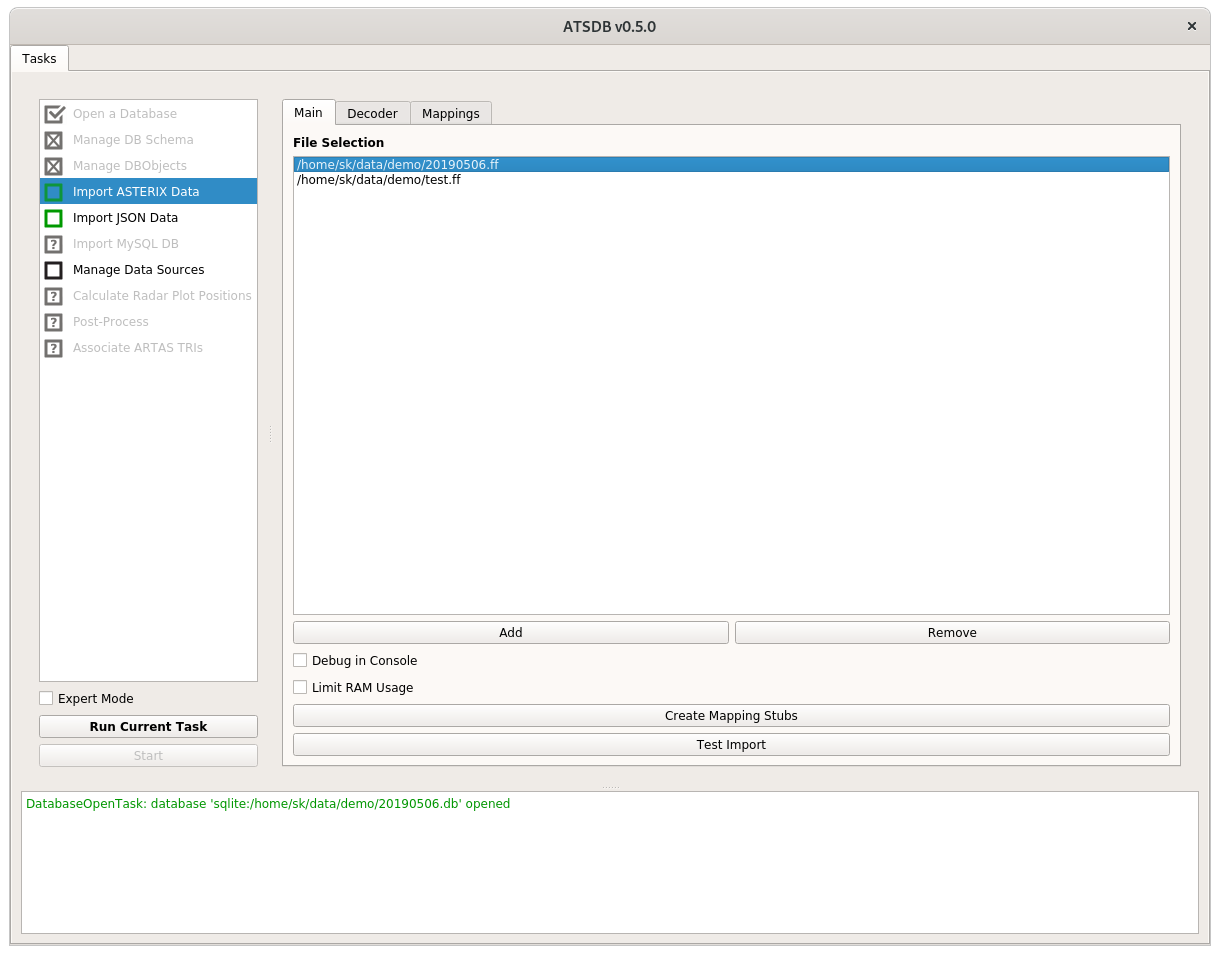
\includegraphics[width=19cm]{../screenshots/asterix_import_data_ready.png}
  \caption{Task: Import ASTERIX data available}
\end{figure}

Using the 'Debug in Console' checkbox, additional debugging information is output to the console, and the ASTERIX decoding is switched to single-threading for easier investigation. \\

Using the 'Limit RAM Usage' checkbox, parallel processing is limited (decreasing RAM usage and processing speed) for usage on smaller workstations. \\

Using the 'Create Mapping Stubs' button, the selected file can be processed and unmapped data entries (which could be mapped to database content) are created in the 'Mappings' definition. \\

Using the 'Test Import' button, the import function can be tested without inserting the data into the 
database, the 'Import' imports the selected file with the given options. This function can be run multiple times. \\

\subsection{Decoder Tab}

\begin{figure}[H]
  \center
    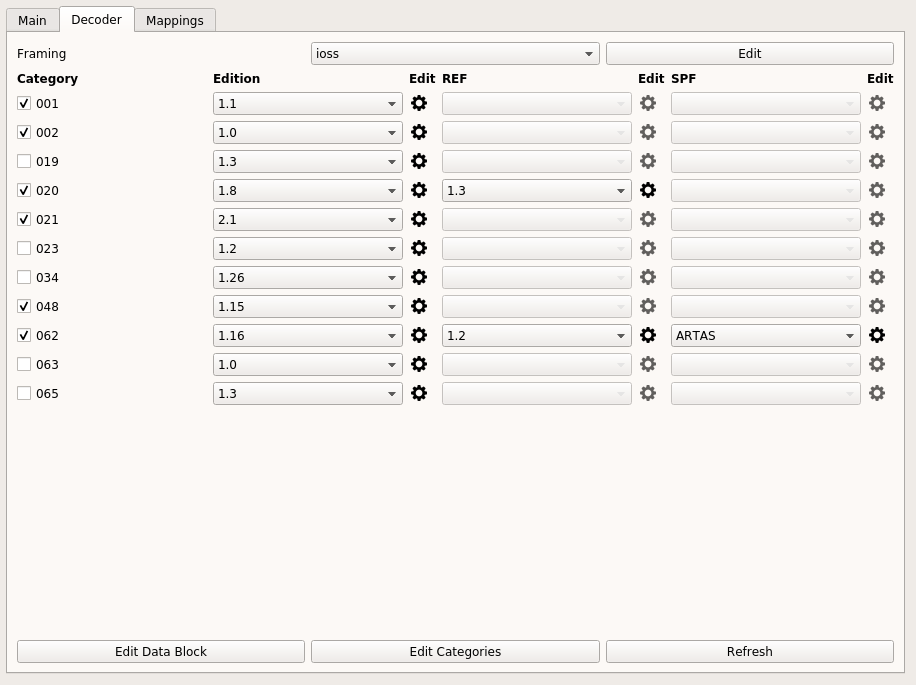
\includegraphics[width=16cm,frame]{../screenshots/asterix_import_data_decoder.png}
  \caption{Task: Import ASTERIX data decoder}
\end{figure}

\paragraph{Framing}
Using the 'Framing' drop-down menu, the current framing can be selected. Using the 'Edit' button, the current framing definition is opened in a text editor.

\paragraph{Categories}

For each category, a number of elements exist:

\begin{itemize}  
\item Category checkbox: Number of category and checkbox defining if it should be decoded
\item Edition: Drop-down menu to select the edition number to be used
\item Edition Edit Button 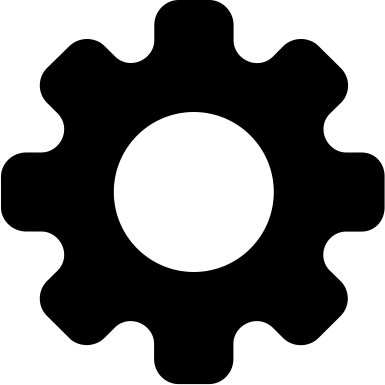
\includegraphics[width=0.5cm]{../../data/icons/edit.png}: Opens the current edition definition in a text editor
\item REF: Drop-down menu to select the Reserved Expansion Field defition (if available)
\item REF Edit Button 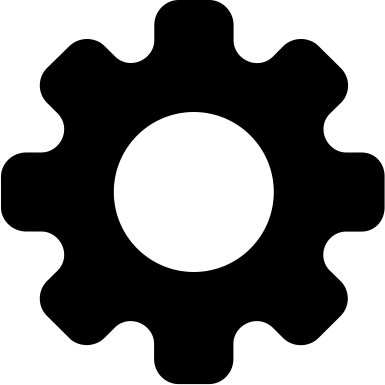
\includegraphics[width=0.5cm]{../../data/icons/edit.png}: Opens the current REF definition in a text editor
\item SPF: Drop-down menu to select the Special Purpose Field defition (if available)
\item SPF Edit Button 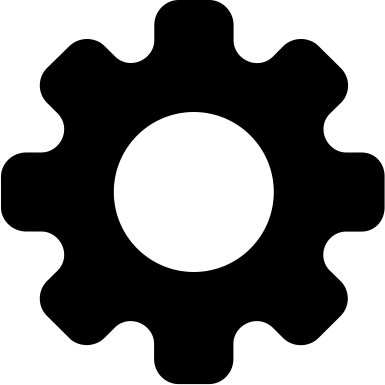
\includegraphics[width=0.5cm]{../../data/icons/edit.png}: Opens the current SPF definition in a text editor
\end{itemize}
\ \\

\paragraph{Additional}

Using the 'Edit Data Block' button, the ASTERIX data block definition is opened in a text editor. \\

Using the 'Edit Categories' button, the ASTERIX definitions file is opened in a text editor. \\

Using the 'Refresh' button, the all of the jASTERIX definitions are re-loaded from the harddisk (e.g. to update after file changes were made). \\

\subsection{Override Tab}
\label{sec:task_import_asterix_override}


\begin{figure}[H]
  \center
    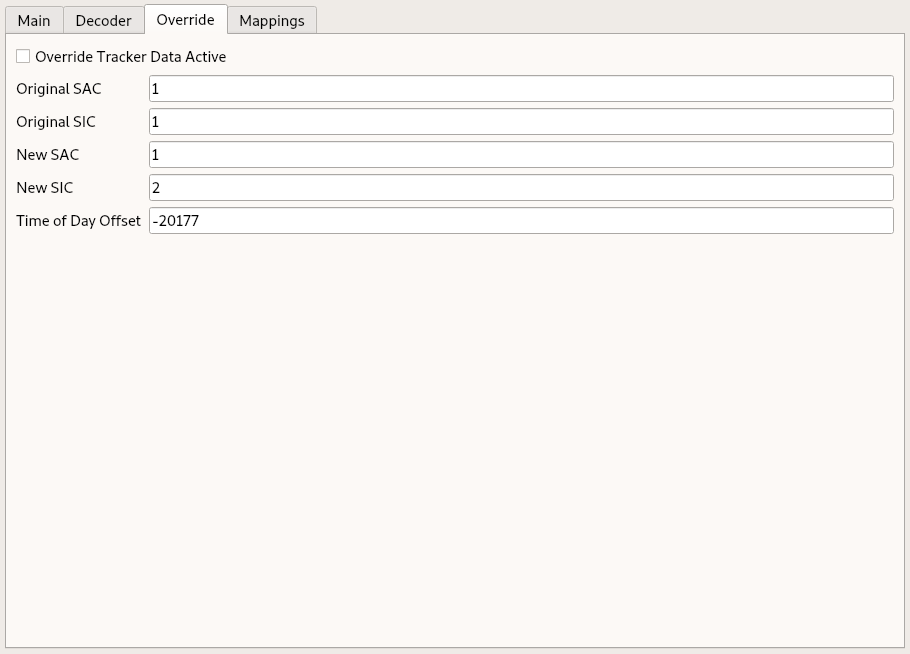
\includegraphics[width=16cm,frame]{../screenshots/asterix_import_data_override.png}
  \caption{Task: Import ASTERIX data override}
\end{figure}

This feature should only be used in very specific circumstances. When activated, the function overrides one specific SAC/SIC in ASTERIX CAT062 data (only) with another value pair, and adds a Time of Day offset. \\

\begin{itemize}  
\item Override Tracker Data Active checkbox: When the override is active. Disabled by default.
\item Original SAC: SAC value for the data source to be overriden
\item Original SIC: SIC value for the data source to be overriden
\item New SAC: New SAC value for the data source
\item New SIC: New SIC value for the data source
\item Time of Day Offset: Positive or negative offset to be added, in seconds. If the resulting value is out of bounds, it is adjusted to the [0, 86400] interval.
\end{itemize}
\ \\

This feature can be used to e.g. import data from different runs of the same tracker, which results in a second dataset with the same SAC/SIC and a time offset. Since this makes analysis more complicated, the override feature can be used. \\

Please \textbf{note} the following points:

\begin{itemize}  
\item Only the data for the original SAC/SIC is overriden, all other data is imported as is.
\item The best way to set the Time of Day Offset is to shift to a time where no midnight crossing occurs
\item The new SAC/SIC can be the same as the original one (if only time should be shifted)
\item The Time of Day Offset can be 0 (if only SAC/SIC should be overriden)
\end{itemize}

\subsection{Mappings Tab}

\begin{figure}[H]
  \hspace*{-2.5cm}
    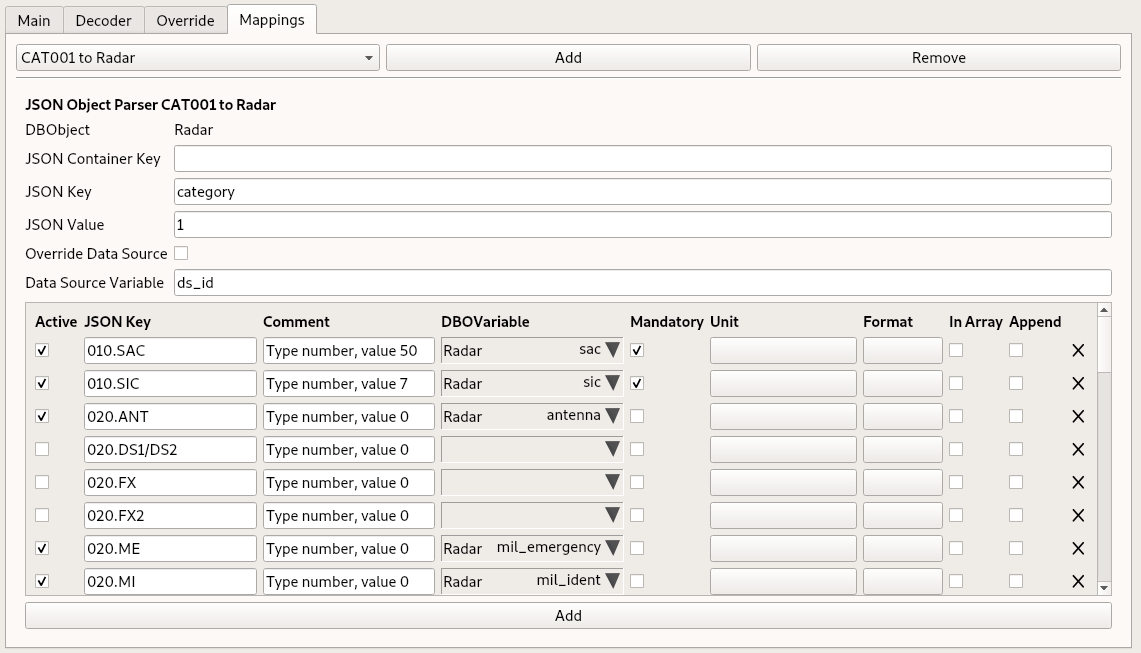
\includegraphics[width=19cm,frame]{../screenshots/asterix_import_data_mappings.png}
  \caption{Task: Import ASTERIX data mappings}
\end{figure}

At the top, the GUI elements can be used to show/add/remove JSON objects parsers. Below that, the currently selected JSON object parser is shown and can be configured. \\

A JSON object parser in this context is the function that parses the JSON content created by the jASTERIX parser, and creates database content from it. For each category a dedicated parser defines the mapping from JSON to database content. \\

For common users normally no interaction is recommended, but it might be sometimes interesting what database content is created from which ASTERIX data.

\paragraph{Top Elements}

Using the drop-down menu, the to-be-shown parser can be selected. The buttons allow for adding and removing JSON object parsers.

\paragraph{Parser GUI Elements}

The exact definition of how the parsing works is out of scope for this document, so only a short summy is given here. For more information please contact the author.


\begin{itemize}  
\item JSON Object Parser Name: Named after the ASTERIX category and the DBObject to which it is mapped
\item Variable List:
\begin{itemize}  
\item Active checkbox: Defines if the specific mapping is used
\item JSON Key: JSON location and name of the data to be mapped, commonly in 'Data Item Number'.'variable' or 'Data Item Number'.'Sub Item'.'variable' format
\item Comment: Additional information with example values
\item DBOVariable: Target variable to which this data is mapped
\item Mandatory checkbox: Defines if the JSON object (from the ASTERIX record) is skipped if the JSON key is not found
\item Unit: Unit and dimension of the JSON data, only defined if conversion is needed
\item Format: Special format of the JSON data, only defined if conversion is needed
\end{itemize}
\end{itemize}
\ \\

\subsection{Running}

Using the 'Run Current Task' button the task can be performed. During import a status indication will be shown:

\begin{figure}[H]
  \center
    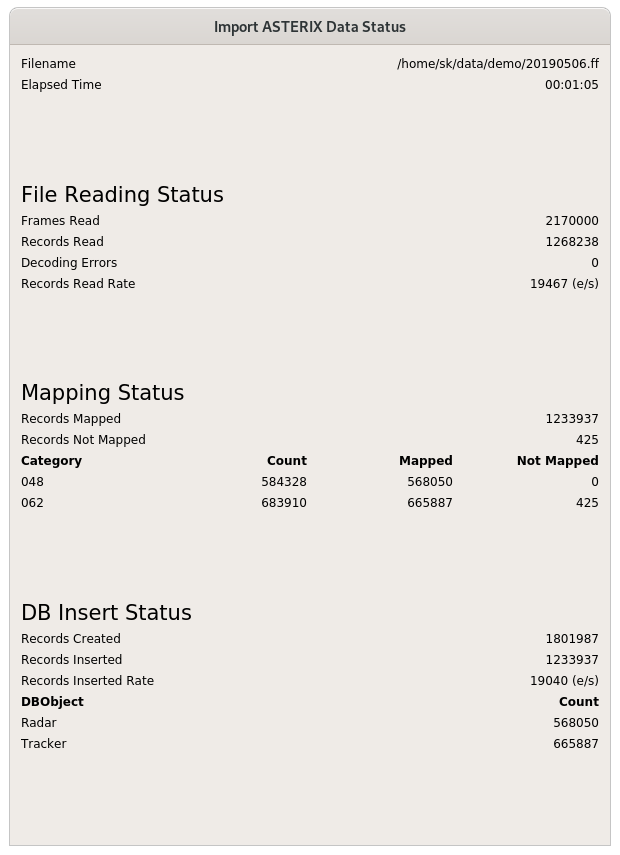
\includegraphics[width=12cm]{../screenshots/asterix_import_status.png}
  \caption{Import ASTERIX data task status}
\end{figure}

If an decoding error occurs, a brief message box is shown, after which the application has to be closed. Please make sure that the correct framing and edition versions are selected, or contact the author for support if this does not resolve the issue. \\

After import, a confirmation will be shown:

\begin{figure}[H]
  \center
    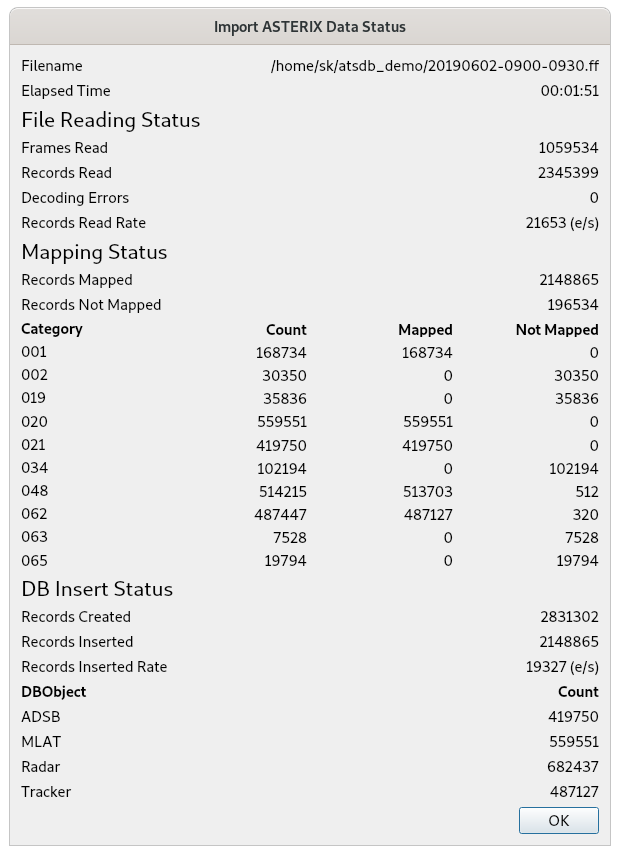
\includegraphics[width=12cm]{../screenshots/asterix_import_done.png}
  \caption{Import ASTERIX data task done}
\end{figure}

\paragraph{Comments}
Importing performance strongly depends on CPU performance (multi-threading very beneficial), but a import of 5 million target reports takes about 3:30 minutes on the author's hardware. \\

The (truncated) timestamps of CAT001 are calculated in a simple algorithm based on the CAT002 messages from the same sensor, so their timestamp data is slightly unreliable, but exact enough for e.g. time window filtering. \\

This task can be run several times, e.g. if multiple ASTERIX recordings from different data sources are to be imported. \\


\includegraphics[width=0.5cm]{../../data/icons/hint.png} Please note the currently not all data fields (as shown in the JSON object parsers) are imported.\\


\includegraphics[width=0.5cm]{../../data/icons/hint.png} After the import it is recommended to re-start the application after executing all tasks, since currently a memory leak during import exists. While this does not cause any issues, usage of the application directly after the import process may be slower than usual for very large datasets. A re-start of the application resolves this issue. \\ 
